\section{Validation and an audit of a published method}\label{sec:exp}

Two questions have to be answered before the decomposition can be used on anything, and
they are answered here in that order. Does the estimator recover what it claims to, with
intervals that cover --- and what, precisely, does it fail to separate?
Section~\ref{sec:simulation} answers both under controlled alternatives where the truth is
known by construction. Then, does it say anything a benchmark's own metrics do not?
Section~\ref{sec:sggaudit} puts it to two publicly released checkpoints of a widely cited
debiasing method, chosen so that the audited models are not ours and the claimed
improvement is one the field already reports. Three further studies --- our own Visual
Genome predictors, a frozen-CLIP variant of them, and long-tailed image and text
classification --- apply the identical estimator and are reported in
Appendix~\ref{app:studies}; Section~\ref{sec:further} summarizes what they add. All
confidence intervals are $95\%$.
\subsection{Controlled validation}\label{sec:simulation}

We generate 24 cells over five labels, drawing each cell's label distribution from
a Dirichlet law and taking the old model to be exactly the cell prior. The new model
interpolates toward an oracle, $q_1=(1-\beta)q_0+\beta q_{\rm oracle}$ with
$q_{\rm oracle}$ placing $0.98$ on the realized label, and forty repetitions are run at
each $\beta\in\{0,.1,\ldots,.8\}$. Across that range the estimated covariance gain grows
linearly and monotonically with the injected signal (Figure~\ref{fig:simulation}, left).

Type-I behaviour is assessed by perturbing the prior predictions with mean-zero noise
and then randomly reassigning the perturbed vectors within each cell, which guarantees
that no systematic prediction--label alignment survives. Over 200 such datasets the
99-shift randomization test rejects in $0.030$ of runs at level $0.05$, with a mean
estimated covariance gain of $-8.97\times10^{-5}$; the null $p$-values come out
approximately uniform and the null estimates stay centred at zero
(Figure~\ref{fig:simulation}, centre and right).

\paragraph{Coverage of the primary interval.} The oracle-signal and null designs above
validate the estimator's centering and the randomization diagnostic, but the paper's
primary uncertainty statement is the image-clustered H\'ajek interval, so we validate
its coverage directly in the regime that stresses it: relations grouped into images
(one to about thirty per image) whose oracle weight shares a latent per-image effect,
and Zipf-distributed cell sizes in which most identified cells hold exactly two
examples. Against the design expectation estimated from 4{,}000 independent
replications, the cluster-robust interval covers in $94.0\%$ of 500 runs, while an
interval that wrongly treats relations as independent covers in only $88.6\%$ --
quantifying both the mild finite-sample undercoverage of the asymptotic interval and
the necessity of clustering.

\paragraph{Discriminant validity.} Three further designs test that the channels
separate what they claim to separate. First, a \emph{calibration-only} alternative:
the new model is a temperature-softened copy of an overconfident informative model, so
the pair contains identical instance information. The raw decomposition credits it with
a large negative covariance gain (mean $-0.488$) -- the confound quantified on real
models in Appendix~\ref{app:lt} -- while the calibration-matched protocol below reduces
it to $-0.0003$ (sd $0.0017$ over 200 runs), confirming that the protocol removes
exactly the confidence-scaling channel. Second, a \emph{prior-only} improvement (the
new model corrects a heteroscedastically noisy estimate of the cell prior, adding no
instance information) yields a covariance gain centred at zero ($0.0002$, sd $0.0035$)
with a clearly positive transported channel: prior improvements do not leak into
$\widehat{\Delta R}$ beyond the algebraic guarantee of Theorem~\ref{thm:population}.
Third, an \emph{unrecorded within-cell shortcut} (a binary feature, varying inside each
cell, that shifts the label distribution and is used by the new model) is credited to
covariance ($+0.041$, sd $0.004$), quantifying the stated limitation that
$\widehat{\Delta R}$ measures all within-cell predictive signal relative to the
declared $\phi$, shortcut or otherwise, and cannot by itself distinguish the two.

\paragraph{The calibration-matched protocol.} The third of those designs identifies a
limitation serious enough to be part of the procedure rather than a caveat about it.
Because $\Delta R$ is a covariance between probability movements and labels
(Theorem~\ref{thm:population}), rescaling a fixed model's confidence moves score between
the two components while adding no information about any individual case: a monotone
transformation of the predictions changes the decomposition even though it changes no
ranking and no decision. We therefore adopt the following control wherever the compared
models differ visibly in confidence. Split the evaluation units --- images, where
examples are clustered --- at random into halves. On the first half, fit each model a
single temperature $T$ by maximum held-out likelihood on $q^{1/T}$ renormalized. On the
second half, apply each model's own fitted temperature and run the decomposition there.
The protocol costs nothing but a data split, it uses no label information from the
audited half, and it is what the simulation above shows removes the confidence-scaling
channel almost exactly.

How many splits each study averages over differs, and the difference is worth stating
rather than glossing. The long-tailed classification study of Appendix~\ref{app:lt}
averages over twenty random splits. The audit of Section~\ref{sec:sggaudit} and the
matched rows of Appendix~\ref{app:vgvisual} each use a single split at a fixed seed. For
those two the split is a source of variability the reported interval does not include, and
it is not negligible: the calibration-only arm above has a between-split standard
deviation of $0.001725$, exceeding the half-width of the audit's own reported interval
($0.00115$). The audit's conclusion does not turn on this --- its estimate is
indistinguishable from zero and stays so under any split --- but a reader comparing
interval widths across our tables should know that two of the three matched studies report
within-split uncertainty only. It does not make $\Delta R$ invariant to recalibration in
general; it fixes the confidence scale at which the comparison is made, which is what a
comparison of two \emph{fixed} models needs.

\begin{figure*}[t]
\centering
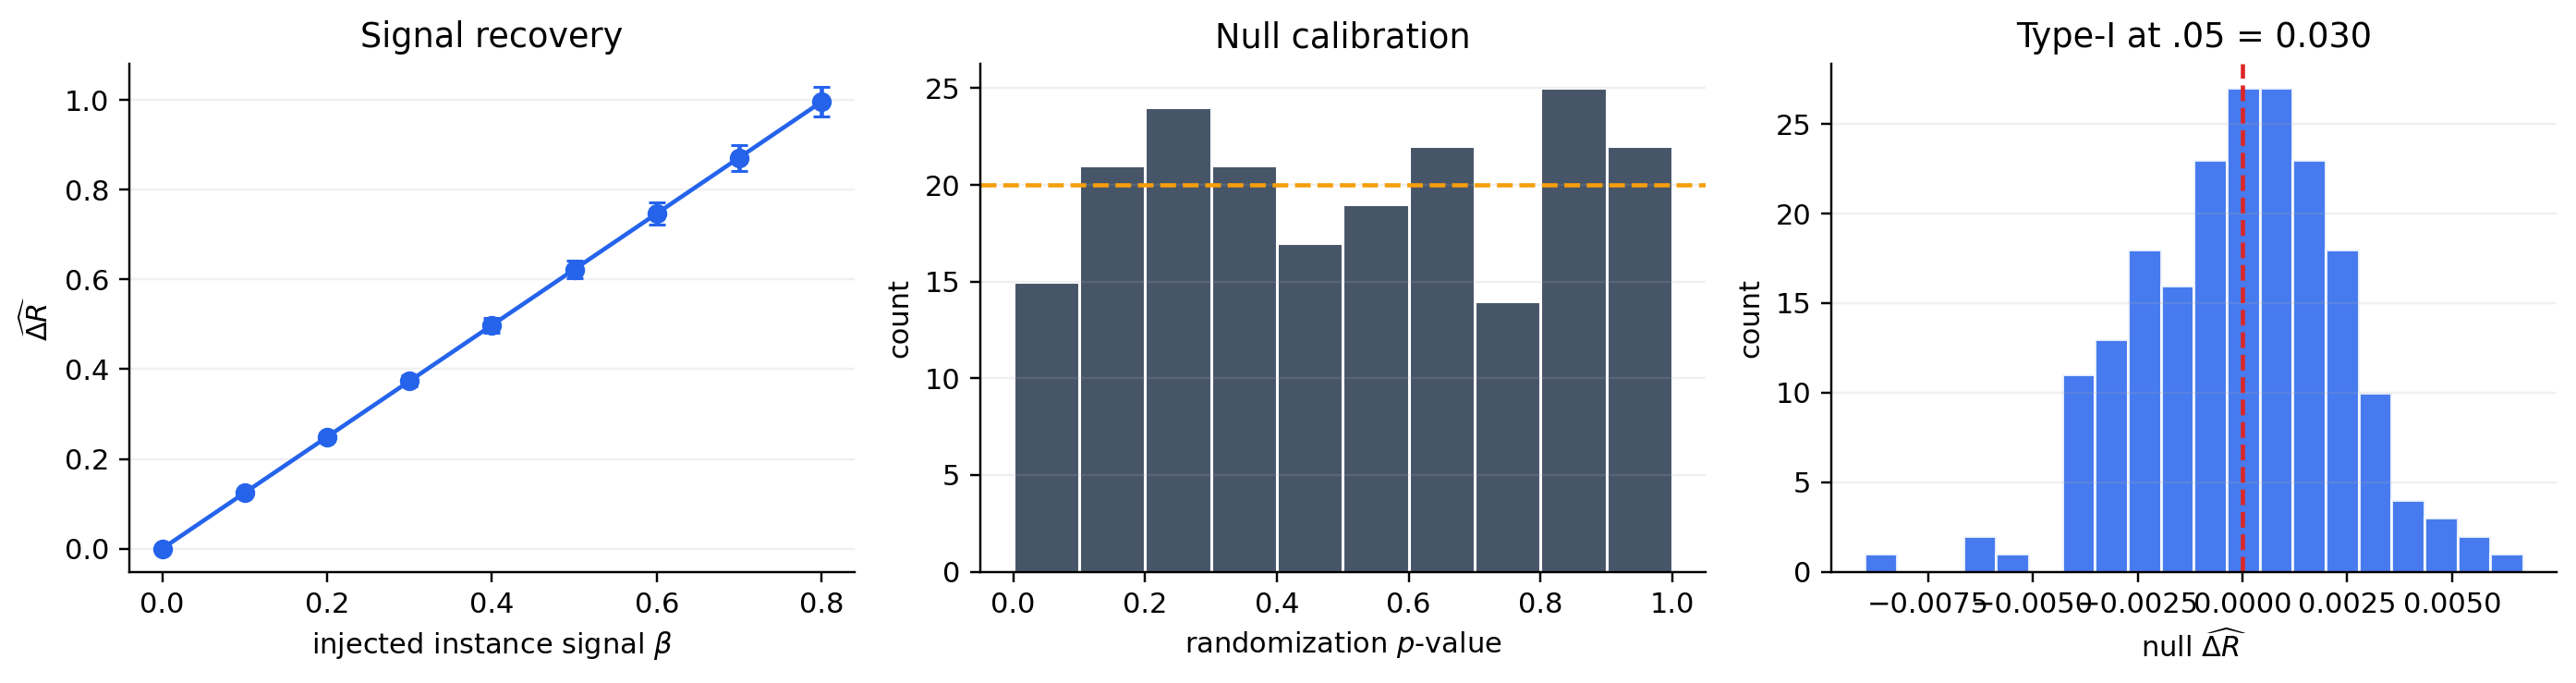
\includegraphics[width=\textwidth]{figures/fig3_new_simulation.png}
\caption{\textbf{Controlled validation.} WAGER recovers injected within-cell signal
monotonically (mean $\pm$ one standard deviation), produces approximately uniform null
randomization $p$-values, and controls type-I error in 200 null runs.}
\label{fig:simulation}
\end{figure*}

\subsection{Auditing a published debiasing method}\label{sec:sggaudit}

The question the decomposition exists to answer concerns systems that other people
release and that the field already compares, so the primary application is to a published
pair rather than to predictors of our own. Tang et al.\ \cite{tang2020unbiased} release a causal MOTIFS PredCls
checkpoint that yields two models from one set of weights: the biased baseline
(MOTIFS-SUM) and its Total Direct Effect counterpart (MOTIFS-TDE), which subtracts a
context-only counterfactual at inference. TDE is among the most cited debiasing methods
in scene graph generation, and it is reported through mean recall, so it is exactly the
kind of claimed improvement whose composition is at issue.

We evaluate both variants with the authors' own code on the canonical VG150 test split,
which fixes the vocabulary, the split and the relation set, and makes the two prediction
sets aligned relation-for-relation by construction. Our reproduction matches the
published behaviour: the baseline reaches $R@50=0.6612$ with $mR@50=0.1459$, and TDE
trades the former for the latter, reaching $R@50=0.4588$ with $mR@50=0.2476$ and raising
zero-shot recall from $zR@50=0.1102$ to $0.1432$. Top-1 predicate accuracy falls from
$0.6981$ to $0.5577$. The audit uses $183{,}639$ relations over $26{,}446$ images and
$7{,}127$ class-pair cells, of which $98.9\%$ are identified.

\paragraph{What is audited, precisely.} One point of bookkeeping before the numbers, since
it changes what the headline row is a statement about. The rows labelled
calibration-matched do not decompose the released checkpoints as released; they decompose
the two models after each has been rescaled by its own temperature ($T^*=2.50$ for the
baseline, $0.92$ for TDE) fitted on a held-out half of the images. That is the comparison
we argue is meaningful, because a proper score punishes miscalibration and these two
models differ sharply in it. But the released pair, scored as it ships, gives a
\emph{significant} covariance loss ($-0.01355$, interval excluding zero), and a
practitioner who downloads those weights and scores them is looking at the raw rows. We
report both and label which is which.

\paragraph{Result.} Table~\ref{tab:sggaudit} decomposes the pair. Read raw, TDE loses
$0.11651$ of quadratic score, of which $0.10296$ sits in the transported channel and a small
but significant $0.01355$ in within-group covariance. That reading does not survive the
control this paper insists on. The two models differ sharply in confidence --- the
baseline is overconfident at $T^*=2.50$ while TDE, having subtracted a counterfactual,
is already near-calibrated at $T^*=0.92$ --- and once temperatures are fitted on a
held-out half of the images and the audit runs on the other half, the quadratic-score
covariance channel is indistinguishable from zero: $\widehat{\Delta R}=-0.00006$ with a
$95\%$ interval of $[-0.00120,+0.00109]$ and a randomization $p$ of $.555$. Essentially
the entire proper-score difference, $-0.18258$ of $-0.18264$, is transported.

The log-score row of the same calibrated comparison does not repeat this null: it
returns $\widehat{\Delta R}=+0.04396$, $95\%$ CI $[+0.04079,+0.04714]$, an interval that
excludes zero. The two proper scores therefore disagree on whether any real covariance
change survives calibration matching -- one reads exactly null, the other reads small
but significantly positive -- while agreeing that whichever value is correct is far
smaller than the calibrated prior-channel shift ($-0.18258$ under the quadratic score,
$-0.59157$ under the log score, both an order of magnitude or more larger than either
covariance estimate). We do not adjudicate between the two scores here: nothing in
Section~\ref{sec:setup} privileges one proper score's covariance estimate as the
``true'' one, and this is the reason the paper's default score is stated as a
declared choice rather than derived. The claim this audit actually supports is the one
both scores agree on --- that TDE's proper-score improvement over the baseline is
overwhelmingly transported \emph{at the calibration-matched, class-pair configuration},
with a covariance remainder at most a small fraction of the total and possibly exactly
zero --- not the stronger, single-score claim that within-group covariance is unchanged.

That qualifier is load-bearing, and we would rather state its force than let a reader
discover it in the table. Table~\ref{tab:sggaudit}'s five configurations of this one pair
give covariance gains of $-0.21711$, $-0.12619$, $-0.01355$, $-0.00006$ and $+0.04396$.
At two of the five, ``overwhelmingly transported'' is simply false: the raw log-score row
has $|\widehat{\Delta R}|=0.126$ against $|\widehat{\Delta P}|=0.159$, and the
subject-only row has $\widehat{\Delta R}=-0.217$ dominating $\widehat{\Delta P}=+0.102$.
We report all five and argue for one on stated grounds --- matched confidence, because a
proper score punishes miscalibration; the finest defensible cell, because
Proposition~\ref{prop:coarsen} makes coarsening non-neutral --- rather than presenting the
favourable configuration as the finding. Theorem~\ref{thm:bregman} is the reason the
score-dependence is not a defect to be argued away: each Bregman generator defines its own
exact estimand, so two proper scores disagreeing about $\Delta R$ are answering two
well-posed questions, and which one an evaluator wants is a declaration, not a fact about
the models.

This is a precise and, we think, fair characterization of what TDE does. Its own
construction subtracts the context-only prediction, so a method that operates on the
transported channel is what its authors built; WAGER quantifies that the intervention is
almost purely of that kind, and that the model's ability to tell which relation belongs
to which image within a class-pair cell is left, at most, only marginally changed. The
consequence for evaluation needs stating carefully, because it is easy to state in a way
that is not quite true. Mean recall rose by $10.2$ points; the quadratic-score covariance
gain, calibration-matched at the class-pair cell, is $-0.00006$ with an interval
containing zero. Those are different units and we have no bridge between them. Nothing
here licenses the claim that ten points of mean recall bought $0.00006$ of case-level
evidence, and it would be equally wrong to say the mean-recall gain \emph{is} transported,
since the transported channel on the proper score \emph{fell} over the same comparison
($\widehat{\Delta P}=-0.18258$). What the audit supports is a conjunction of two separate
statements: the field's headline metric moved ten points, and the proper-score difference
between the same two models decomposes almost entirely into the transported channel, with
a covariance remainder at most a small fraction of it. A reader may conclude that the
metric movement is not evidence about within-cell case-level discrimination, because the
quantity that would measure that barely moves. A reader may not conclude a conversion
rate, and we do not supply one.

One further qualification: TDE is designed to change the decision rule rather than to
emit calibrated probabilities, and a proper score evaluates the latter; the
calibration-matched regime is what makes the comparison meaningful at all, and its
necessity here is the clearest practical argument for the protocol of
Section~\ref{sec:simulation}.

\begin{table}[t]
\centering
\caption{WAGER audit of released checkpoints on the canonical VG150 PredCls split:
MOTIFS-TDE against the MOTIFS-SUM baseline it debiases, both evaluated with the
original authors' code. Raw rows use all identified relations; the calibration-matched
rows fit each model's temperature on a held-out half of the images and audit the
disjoint half. CI is image-cluster robust on $\widehat{\Delta R}$.}
\label{tab:sggaudit}
\resizebox{\textwidth}{!}{%
\begin{tabular}{@{}lllrrr@{}}
\toprule
Regime & Score & Cell $\phi$ & $\widehat{\Delta T}$ & $\widehat{\Delta P}$ &
$\widehat{\Delta R}$ (95\% CI) \\
\midrule
raw & quadratic & class pair & $-0.11651$ & $-0.10296$ & $-0.01355\,[-0.01504,-0.01206]$ \\
raw & log       & class pair & $+0.03277$ & $+0.15897$ & $-0.12619\,[-0.13093,-0.12145]$ \\
raw & quadratic & subject    & $-0.11536$ & $+0.10175$ & $-0.21711$ \\
\midrule
calibration-matched & quadratic & class pair & $-0.18264$ & $-0.18258$ & $-0.00006\,[-0.00120,+0.00109]$ \\
calibration-matched & log       & class pair & $-0.54760$ & $-0.59157$ & $+0.04396\,[+0.04079,+0.04714]$ \\
\bottomrule
\end{tabular}
}
\end{table}


\subsection{Three further studies, in brief}\label{sec:further}

The audit above uses models we did not build, which is the right test of usefulness but
the wrong test of what the two components mean, since the ground truth about a released
checkpoint is unavailable. Three further studies supply that complementary evidence with
predictors whose information content is controlled by construction. They are reported in
full in Appendix~\ref{app:studies}; what they add is the following.

\emph{Controlled predictors on Visual Genome} (Appendix~\ref{app:vgmain}). Five
predictors that differ only in the features they see are compared pairwise on
$227{,}337$ identified test relations. The decomposition assigns a class-only model's
entire gain over a frequency table to the prior component --- exactly zero covariance
gain, with a zero-width interval, as the construction requires --- while crediting the
addition of box geometry with a covariance gain of $0.01439$ that no aggregate score
separates out. Appendix~\ref{app:vgmain} also reports the granularity, score and
minimum-cell-size sensitivities, including the coarsening that
Proposition~\ref{prop:coarsen} predicts and Table~\ref{tab:sensitivity} measures.

\emph{Real pixels against a geometric proxy} (Appendix~\ref{app:vgvisual}). Replacing box
geometry with a frozen CLIP encoder produces the sharpest case for separating the
components. By every aggregate measure the resulting model is the worst of the three: it
scores $0.04655$ below the geometry model and three accuracy points lower, and an
evaluator reading either number would discard it. The decomposition places its entire
deficit in the prior component while its covariance gain is significantly
\emph{positive}, and that advantage survives both post-hoc prior correction and
calibration matching.

\emph{Long-tailed classification, in images and in text} (Appendix~\ref{app:lt}). The
same estimator, unchanged, is applied to CIFAR-100-LT across seeds and imbalance ratios
and to a long-tailed 20-Newsgroups split, using coarse superclasses and topics as $\phi$.
On CIFAR-100-LT, two standard re-weighting schedules turn out to have opposite
compositions, and the calibration-matched reading reverses what the raw scores suggest
about both: the schedule whose aggregate score barely moves has in fact lost within-class
discrimination, and the one that improves has bought covariance rather than the prior
refit its raw decomposition implies.

The text study is weaker evidence than the CIFAR one and should not be read alongside it
as corroboration. It rests on a single trained pair per schedule, and --- the material
point --- it has no calibration-matched row at all, because no temperature was fitted for
it. Since CIFAR is precisely where we show that recalibration alone can move the channels
by more than the entire size of the text-domain finding, an unmatched result cannot
confirm a matched one. Its composition is also $\phi$-dependent in a way worth stating
here rather than only in the appendix: the deferred schedule's covariance gain reads
$+0.00155$ and indistinguishable from zero at the superclass cell, but $-0.00901$ and
significantly \emph{negative} at the coarser tier partition. We report it as a
demonstration that the estimator runs unmodified on a third data modality and returns
interpretable output, which is all a single unmatched run can support.
